\chapter{Results}\label{chapter:results}

In this thesis, we are not looking to obtain the best possible combination of hyperparameters for training loss or model accuracy.
Instead, we want to observe the effects on training with Hivemind when tuning common hyperparameters such as batch size and learning rate and Hivemind hyperparameters such as the TBS.

Thus, what follows in this chapter are experiments aimed to test the limits and performance of Hivemind training rather than looking for the best model.

\section{Baseline runs}

We begin this chapter by showing the results that we have obtained with the baseline runs.
As mentioned previously in \autoref{chapter:setup}, all baseline experiments are executed on machines with the same configuration, and the total number of samples processed is always the same.
\autoref{table:baseline-experiments-results-GAS-1} lists the average runtimes for baseline runs in minutes.

\footnotesize
\begin{tabularx}{\linewidth}{ |c|c|c|c|c| }
    \caption{
        Average runtimes of baseline experiments in minutes, with the standard deviation amongst reruns in parenthesis.
    }\label{table:baseline-experiments-results-GAS-1}                                 \\
    \hline
    \multicolumn{5}{|c|}{Baseline experiments}                                        \\
    \hline
    Maximum Steps & Batch Size & Learning Rate & Grad. Acc. Steps & Runtime (minutes) \\
    \hline
    2500 & 128 & 0.001 & 1 & 391.2 ($\pm 13.63$) \\
\hline
2500 & 128 & 0.01 & 1 & 399.13 ($\pm 9.93$) \\
\hline
2500 & 128 & 0.1 & 1 & 421.21 ($\pm 4.89$) \\
\hline
5000 & 64 & 0.001 & 1 & 376.42 ($\pm 11.41$) \\
\hline
5000 & 64 & 0.01 & 1 & 371.93 ($\pm 9.09$) \\
\hline
5000 & 64 & 0.1 & 1 & 366.21 ($\pm 1.67$) \\
\hline
10000 & 32 & 0.001 & 1 & 371.62 ($\pm 17.99$) \\
\hline
10000 & 32 & 0.01 & 1 & 364.7 ($\pm 4.78$) \\
\hline
10000 & 32 & 0.1 & 1 & 378.78 ($\pm 8.16$) \\
\hline
2500 & 128 & 0.001 & 2 & 168.87 ($\pm 0.06$) \\
\hline
2500 & 128 & 0.01 & 2 & 166.86 ($\pm 0.06$) \\
\hline
2500 & 128 & 0.1 & 2 & 165.38 ($\pm 0.04$) \\
\hline
5000 & 64 & 0.001 & 2 & 367.96 ($\pm 6.68$) \\
\hline
5000 & 64 & 0.01 & 2 & 374.17 ($\pm 8.1$) \\
\hline
5000 & 64 & 0.1 & 2 & 372.1 ($\pm 7.6$) \\
\hline
10000 & 32 & 0.001 & 2 & 383.8 ($\pm 4.3$) \\
\hline
10000 & 32 & 0.01 & 2 & 382.22 ($\pm 4.49$) \\
\hline
10000 & 32 & 0.1 & 2 & 380.76 ($\pm 2.83$) \\
\hline
    \hline
\end{tabularx}
\normalsize

There are several things that we have to keep in mind while looking at the performance of baseline runs.
First of all, in the baseline runs there is no distributed training happening, and Hivemind features are all turned off.
However, in figure \autoref{fig:net-recv_GAS-1} we can notice by looking at the network metrics that there is an activity in the network of every baseline run.
On average, every machine receives a constant 1.5 MB/s of data on its network.
This may be due to several factors, such as KVM management data, OpenNebula pings, and CEPH data.

In the Setup section, we also introduced our monitoring tool of choice \textit{wandb}.
Because this is an online monitoring tool, some data about our runs is periodically sent to the Weights and Biases server for storage and visualizations.

In \autoref{fig:net-sent_GAS-1}, which shows the bandwidth used for send operations across all baseline runs, we can observe the bandwidth in MB/s used for each run.
On average, this is roughly 0.02 MB/s on every run, a value that can be mostly attributed to \textit{wandb} and other background monitoring operations such as OpenNebula.

In future sections, we will always account for these effects when performing comparisons with baseline runs.

\begin{figure}[h]
    \centering
    \caption{Network bandwidth received for baseline runs with gradient accumulation steps $=1$.}
    \label{fig:net-recv_GAS-1}
    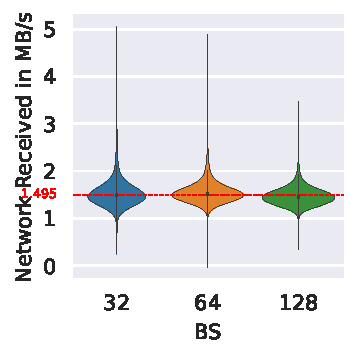
\includegraphics[width=\textwidth]{./figures/06_net-recv_baseline-16vCPUs-GAS-1.pdf}
\end{figure}

\begin{figure}[h]
    \centering
    \caption{Network bandwidth sent for baseline runs with gradient accumulation steps $=1$.}
    \label{fig:net-sent_GAS-1}
    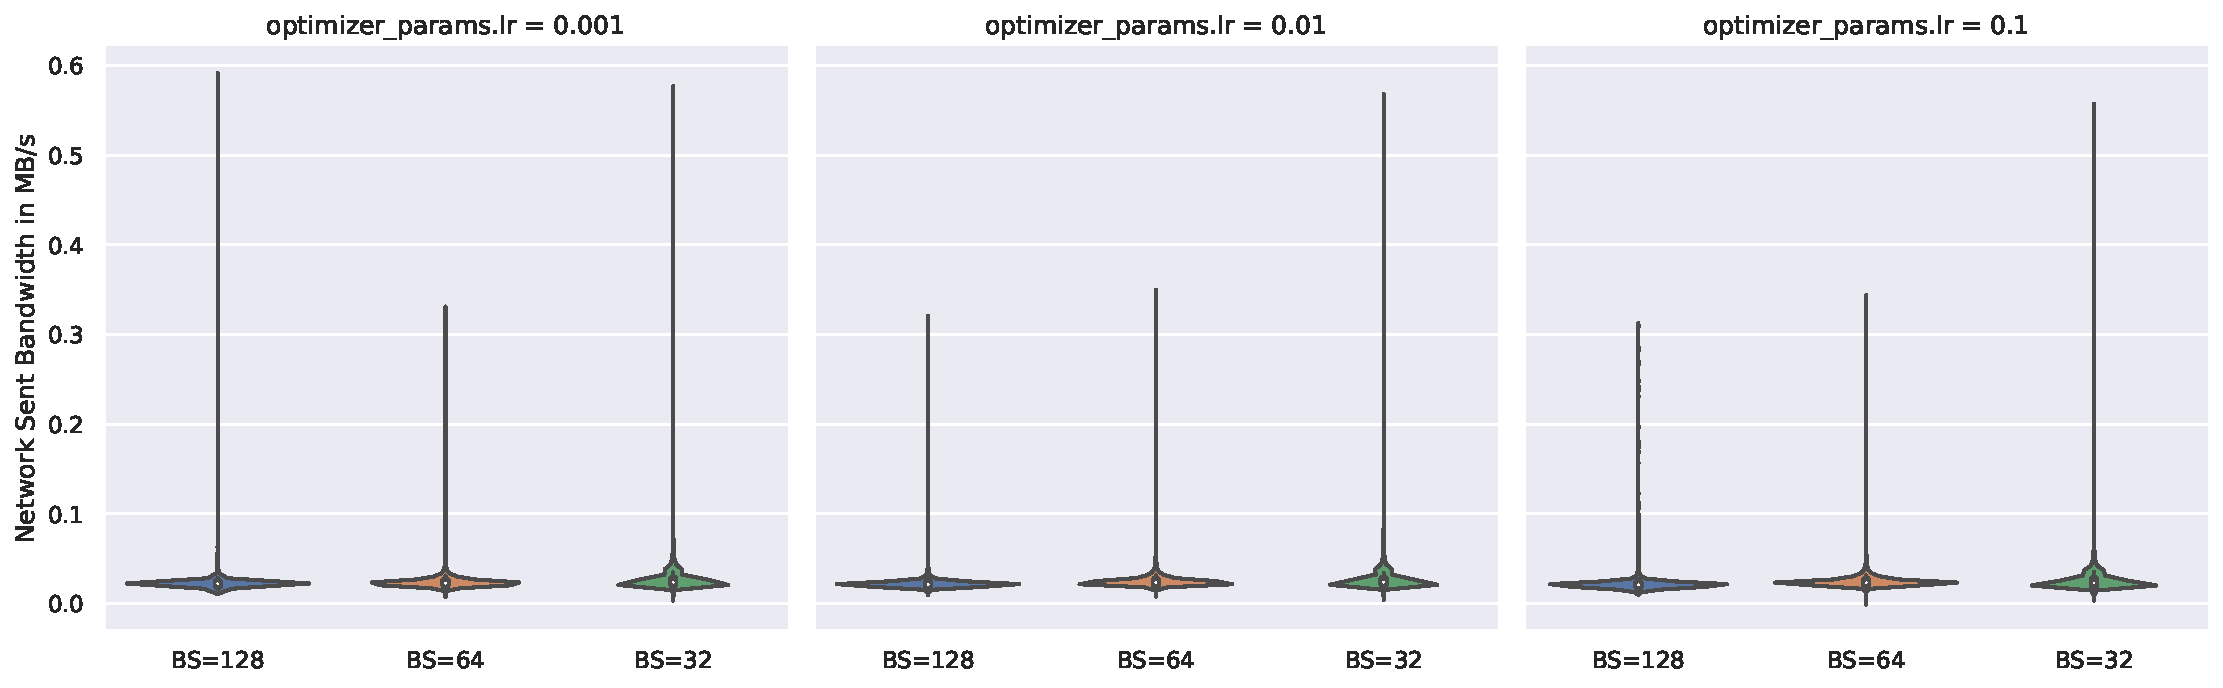
\includegraphics[width=\textwidth]{./figures/06_net-sent_baseline-16vCPUs-GAS-1.pdf}
\end{figure}

\section{Focus on effects of batch size, learning rate and target Batch Size}

Batch size and learning rate are some of the most fundamental hyperparameters to tune when training a neural network to obtain good training results.
Tuning the learning rate should not impact training performance directly, but it can help to better understand how to tune it for different settings combinations while using Hivemind.
As specified in \autoref{chapter:setup}, the reference optimizer algorithm is the stochastic gradient descent (SGD), and the

The batch size determines how many samples are being processed in a training loop.
In Hivemind, this has the consequence of reaching the TBS in fewer steps, but not necessarily in less time.

\autoref{table:use-local-updates_true-GAS-1} shows the runtimes for Hivemind experiments with 2 peers and 8vCPUs per peer compared to the baseline runs.
Every run shows a substantial decrease in runtime by an average of 30\%.
This seems very good at a first glance because it would indicate that we might be able to shave off runtime by almost $1/3$ when turning Hivemind on.
However, there are two important factors to take into consideration before making a such claim:
\begin{enumerate}
    \item Every Hivemind experiment in \autoref{table:use-local-updates_true-GAS-1} fails to reach or decrease the minimum loss established by the baseline runs.
    \item (NOTE: plot something to back this, like a stacked chart or smth) Data loading in the baseline runs takes 1/3 of the total time per step.
\end{enumerate}

\footnotesize
\begin{tabularx}{\linewidth}{ |c|c|c|c|c|c|c|  }
    \caption{
        Runtimes and minimum loss values by Hivemind experiments using 2 peers and 8vCPUs.
    }\label{table:use-local-updates_true-GAS-1}  \\
    \hline
    MS & BS & LR & TBS & GAS & Runtime (minutes) & Loss (min) \\
    \hline
    % see: https://tex.stackexchange.com/a/432308
    \csname @@input\endcsname figures/06_summary-use-local-updates_true-GAS-1
    \hline
\end{tabularx}
\normalsize

\begin{figure}[h]
    \centering
    \caption{Network bandwidth received for baseline runs with gradient accumulation steps $=1$.}
    \label{fig:net-recv_UL-1_GAS-1}
    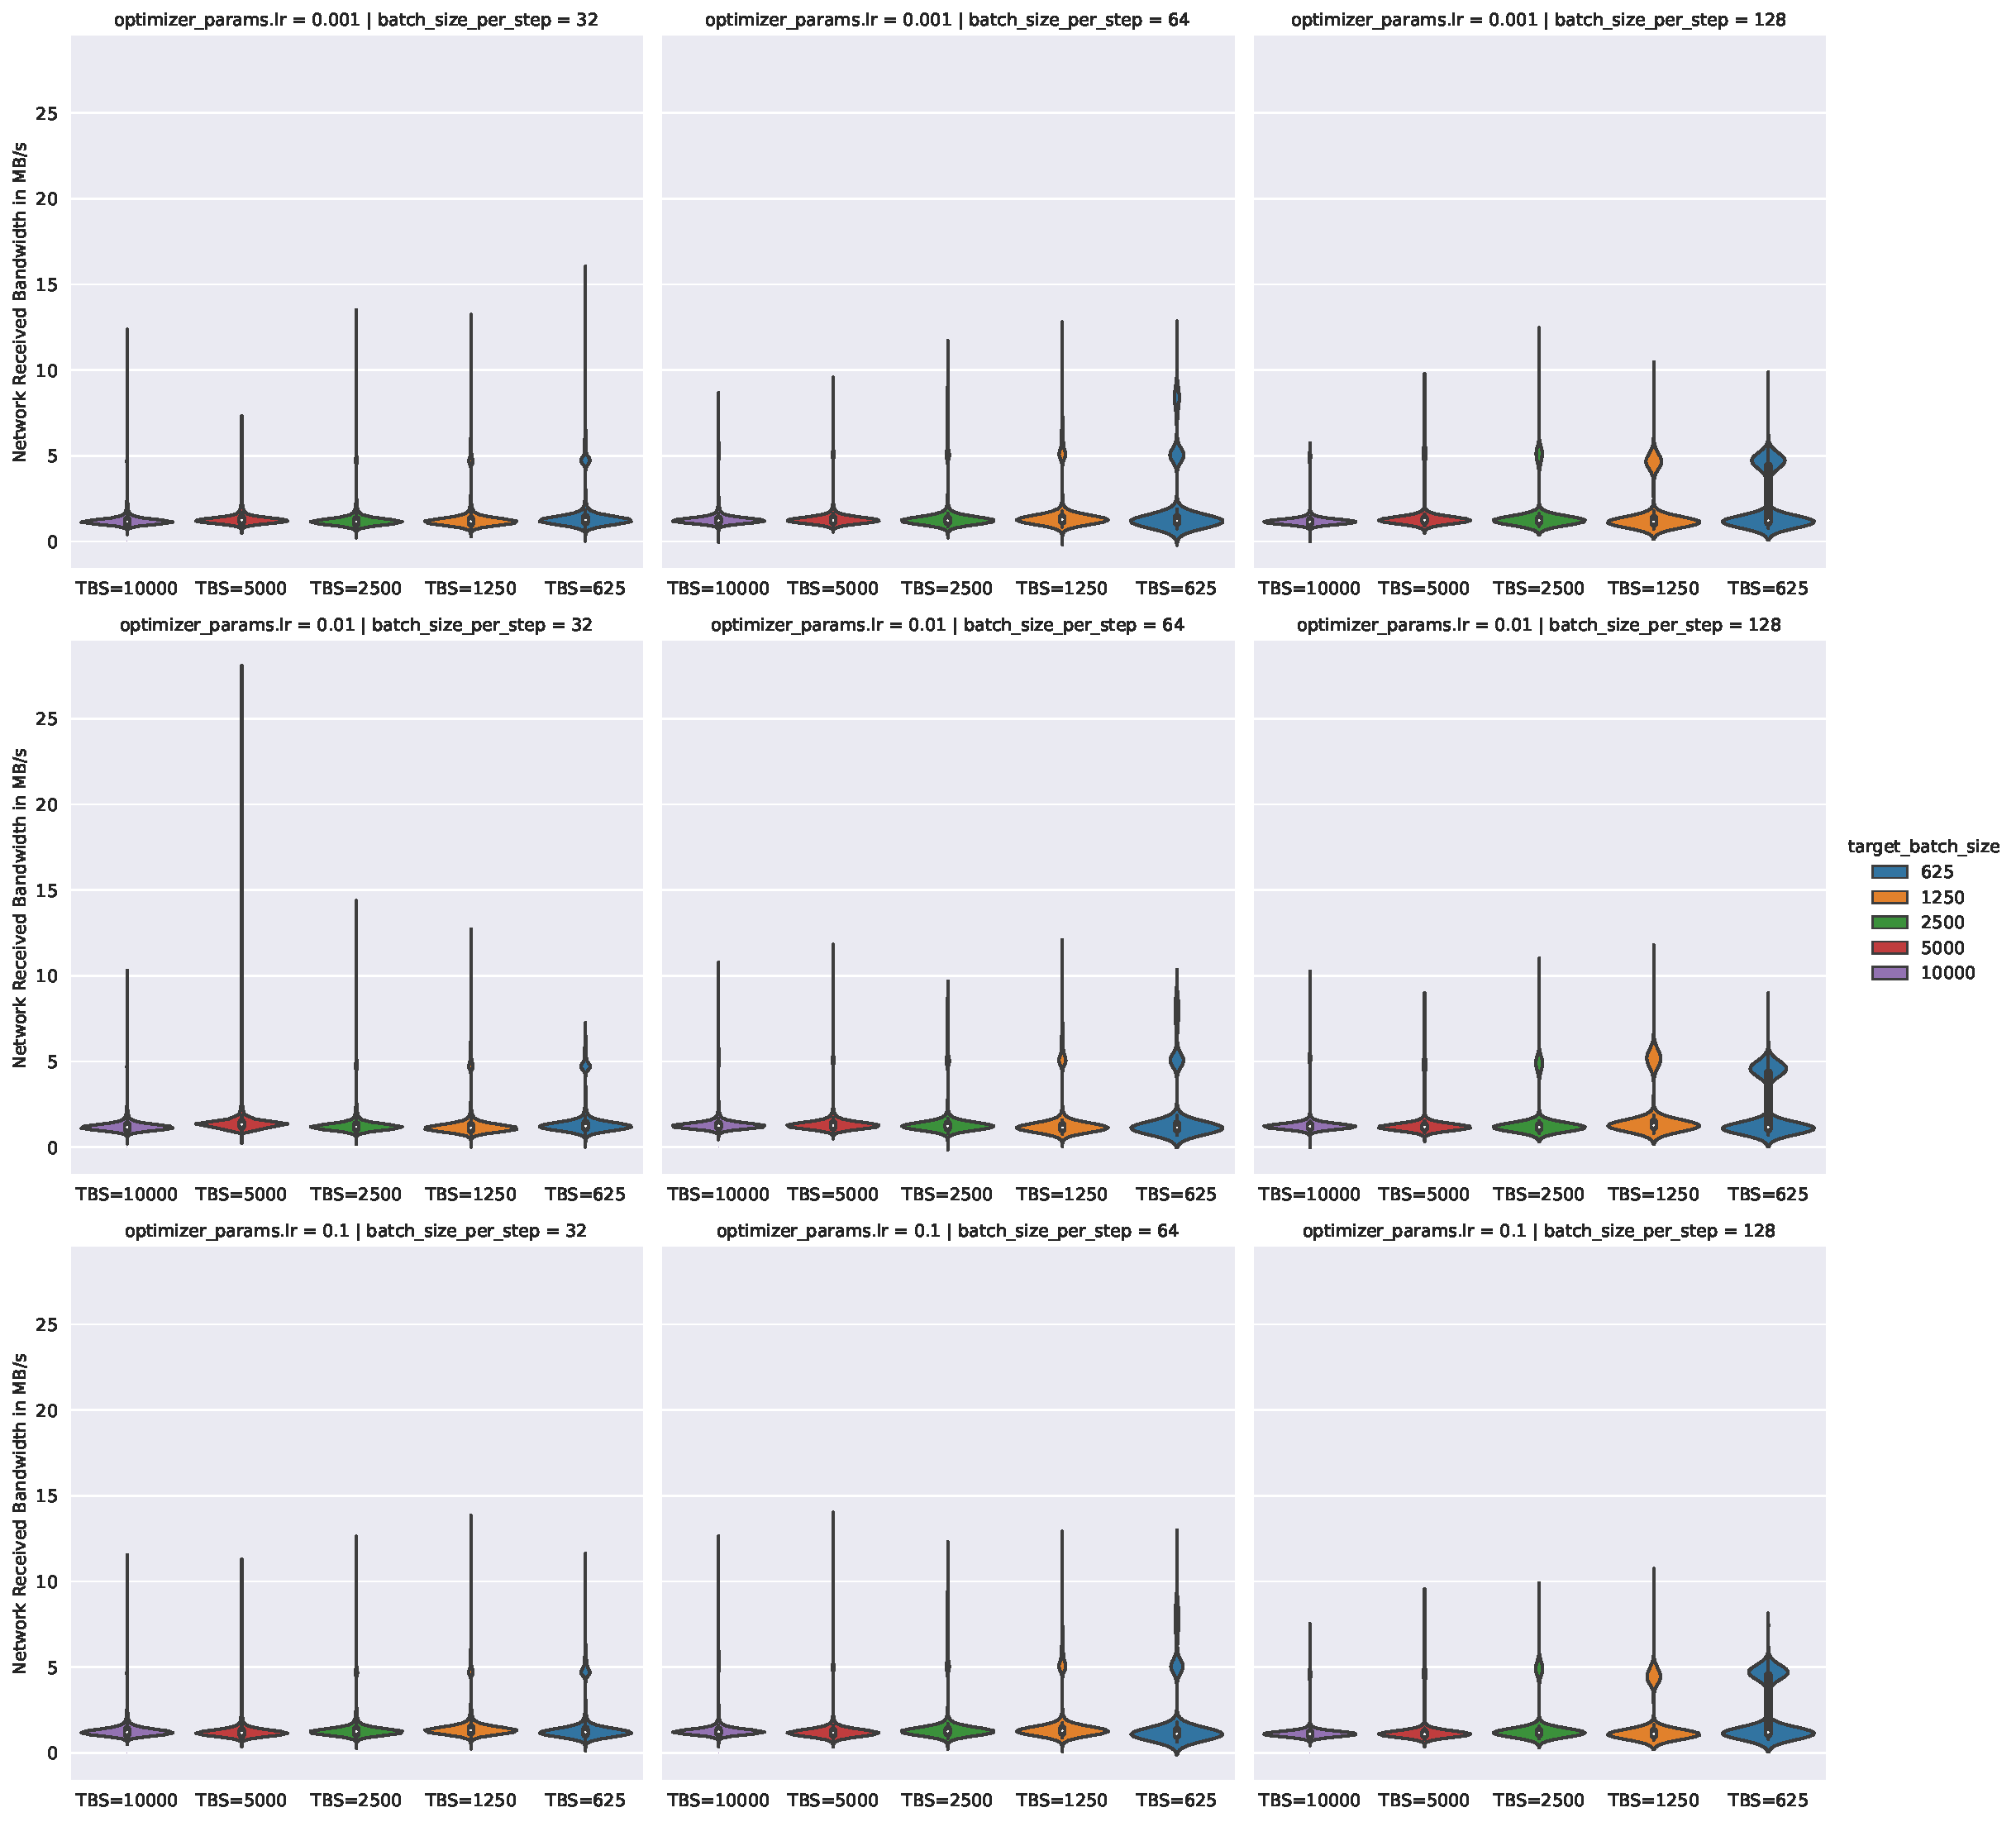
\includegraphics[width=\textwidth]{./figures/06_net-recv-sys-bandwidth-mbs_use-local-updates_true-GAS-1.pdf}
\end{figure}

\begin{figure}[h]
    \centering
    \caption{Network bandwidth sent for baseline runs with gradient accumulation steps $=1$.}
    \label{fig:net-sent_UL-1_GAS-1}
    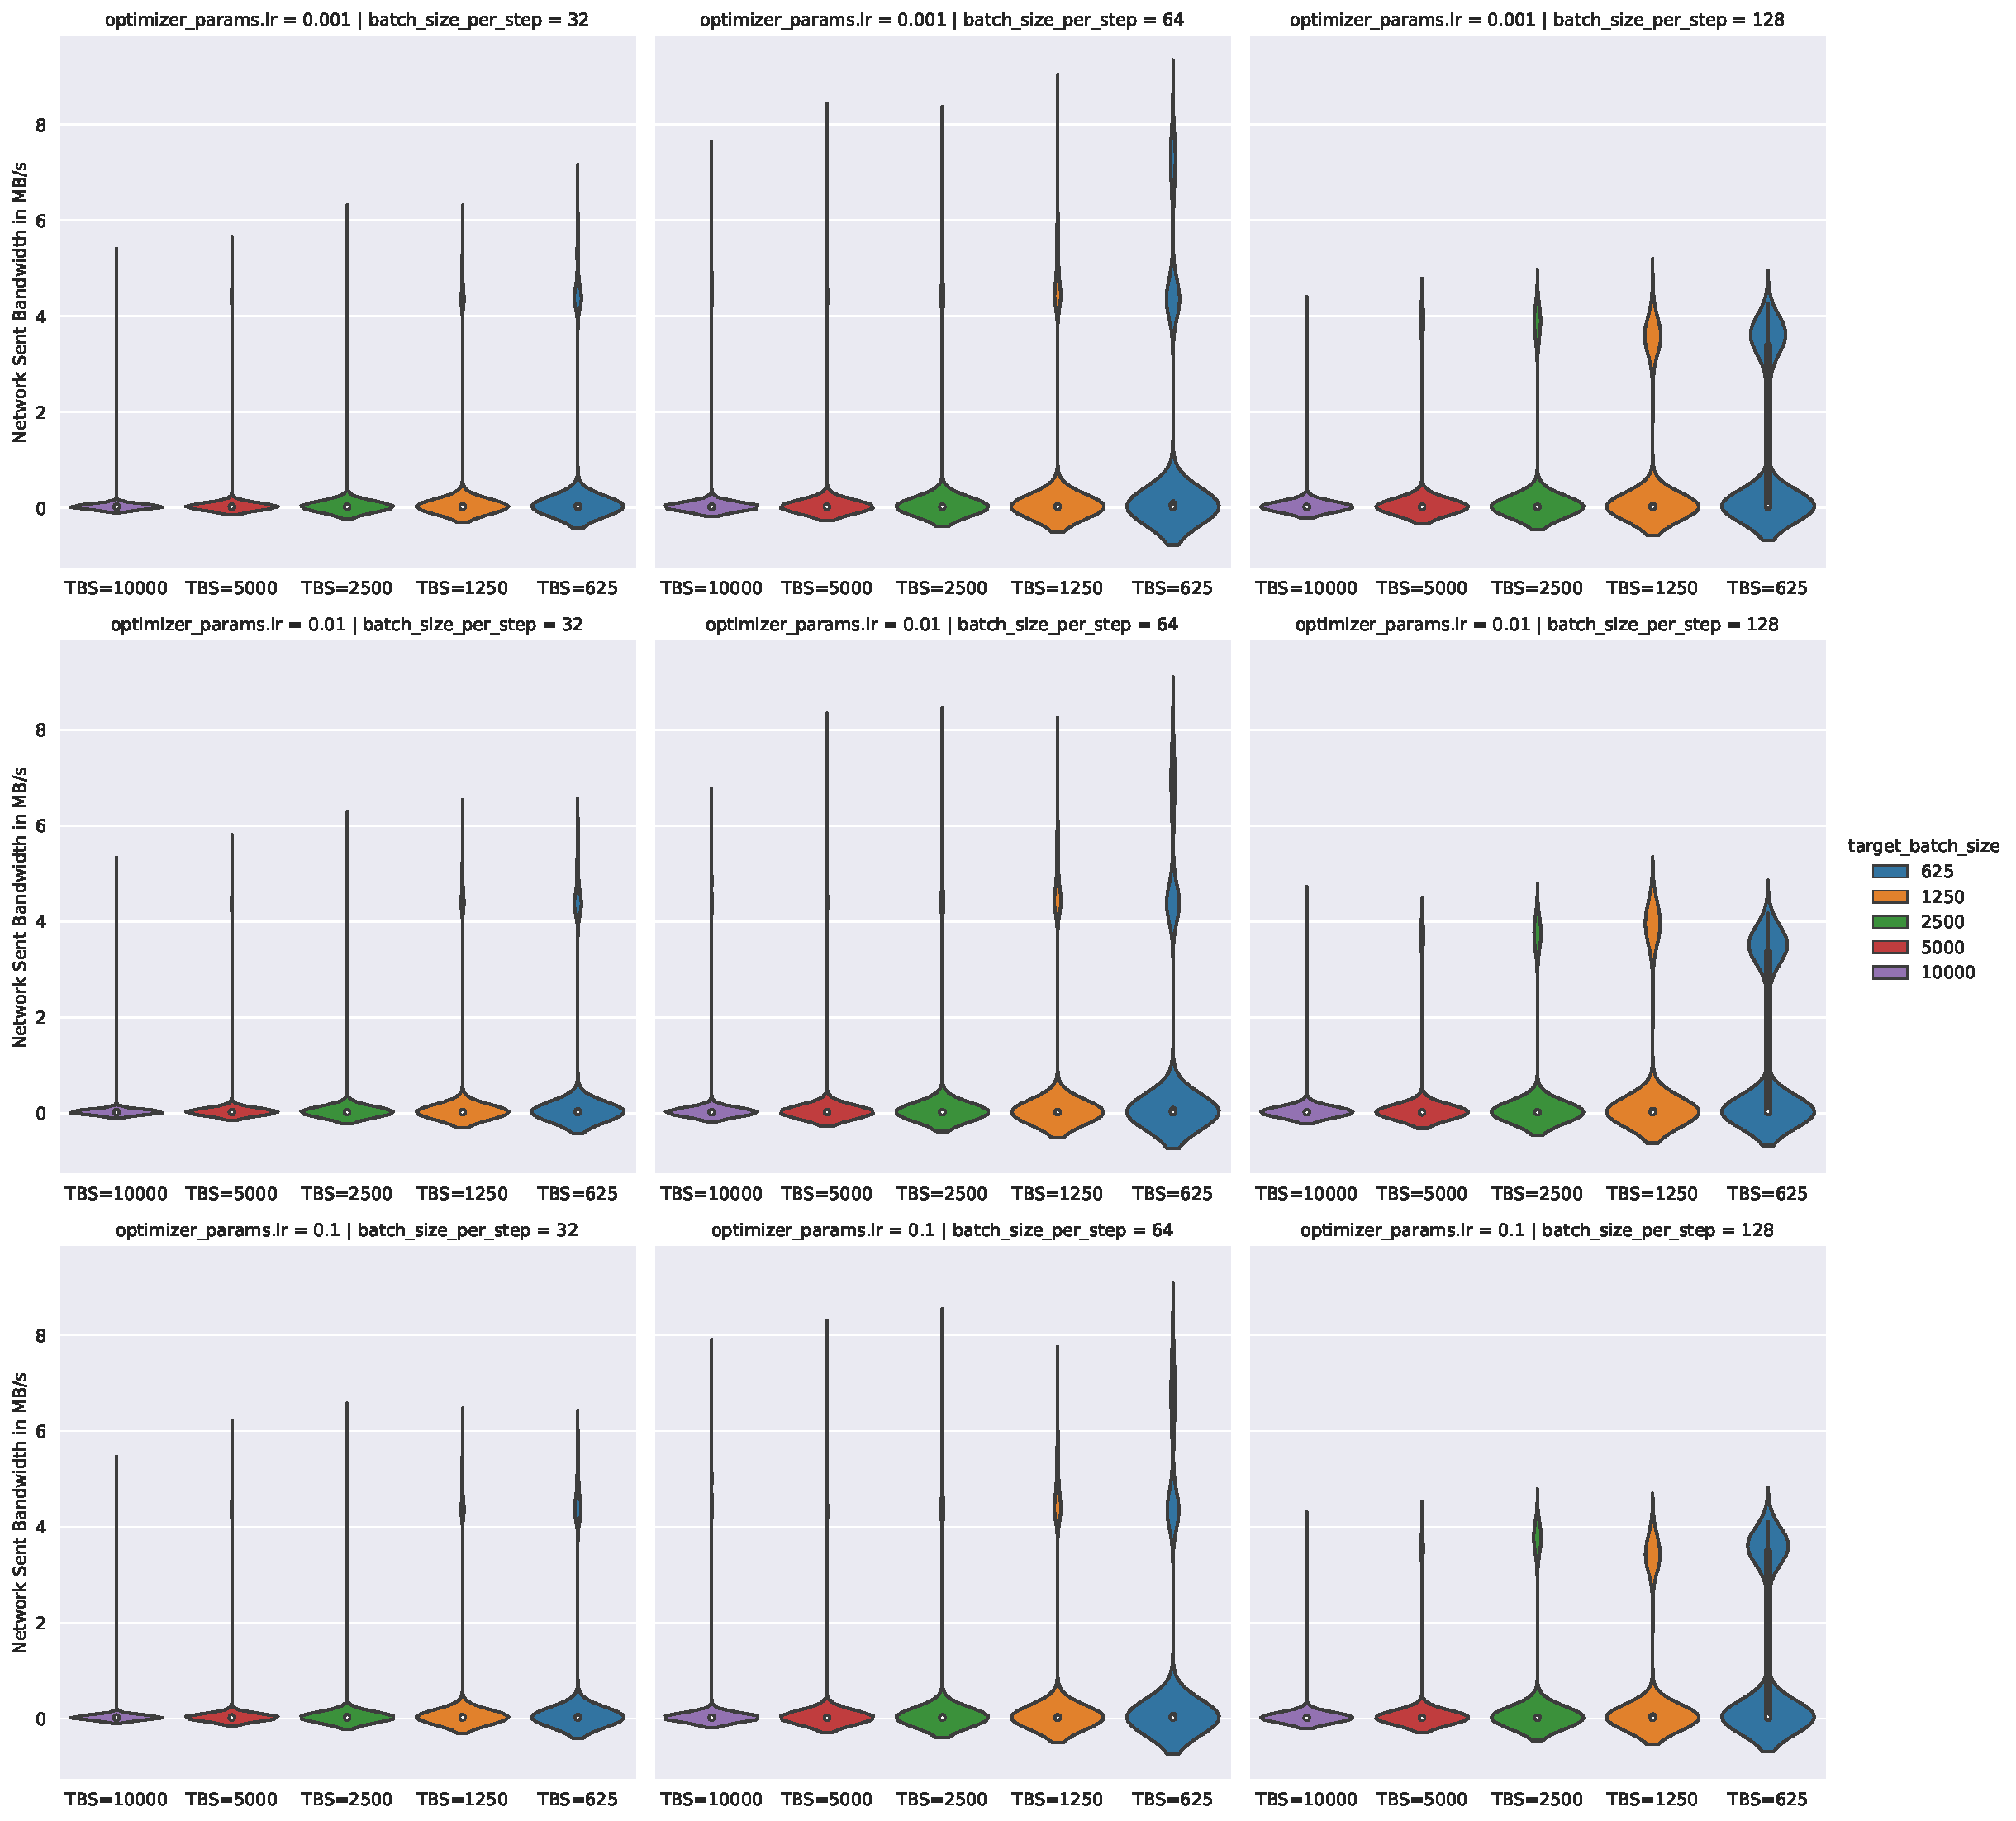
\includegraphics[width=\textwidth]{./figures/06_net-sent-sys-bandwidth-mbs_use-local-updates_true-GAS-1.pdf}
\end{figure}

Considerations of training with Hivemind for the target batch size, batch size and learning rate hyperparameters:

\begin{itemize}
    \item With the same amount of computational power overall, training with Hivemind might need more time to reach the loss from the baseline runs.
    \item Having access to less powerful hardware still allows training peers to be helpful.
    \item Increasing the frequency of averaging does not make up for a bad selection of optimization hyperparameters such as the batch size and learning rate.
    \item However being able to perform averaging steps more frequently can help to reduce the loss gap with the baseline runs.
\end{itemize}

\section{Focus on effects of Gradient Accumulation}

\section{Focus on effects of Local Updates}

\section{Focus on effects of Number of Peers}
